The following three types of image filters have been designed:
\begin{itemize}
    \item Red-Filter
    \item Green-Filter
    \item Blue-Filter
\end{itemize}

These simple filters read pixel data from an \gls{axi} interface and filter out
all channels except one. For example: The red filter filters out everything except the red channel.
\Cref{fig:imagefilter} describes the principle of the filter functionality.
The logic of these filters is connected to the \gls{axi}-Lite Bus.
All three filters share a common Wrapper-Interface and are accessible by a
common Linux-Device-Driver.

\begin{figure}[htbp]
    \centering
    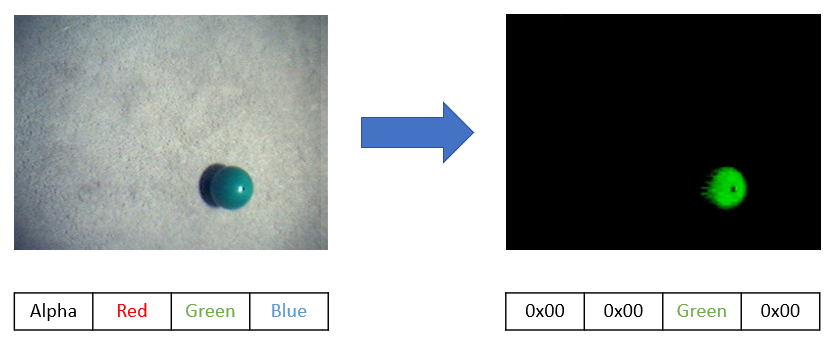
\includegraphics[width=1\textwidth]{images/ImageFilter.PNG}
    \caption{\label{fig:imagefilter} Green Filter example}
\end{figure}

The different cores are added to the system design via the concept described in
\cref{sssec:partialreconfigurationsetup} at the address $0x98000000$ with
the size of $64K$.
The logic behind the common wrapper uses 2 software accessible registers, each
32-bit wide:

\begin{tabular}{ll}
	Address & Name \\
	base     & write\_reg\\
	base + 4 & read\_reg\\
\end{tabular}
\medbreak

The value of the write\_register is processed by the synthesised filter logic
and the result is written to the read\_register.
The related Linux device driver (see \cref{sssec:linuxkernelmodules}) iterates over
the raw \gls{rgb} data written to the device driver file and stores the filtered
data which can then be read back from the device driver file.
